\documentclass[10pt,twocolumn,letterpaper]{article}

\usepackage{iccv}
\usepackage{times}
\usepackage{epsfig}
\usepackage{graphicx}
\usepackage{amsmath}
\usepackage{amssymb}

% Include other packages here, before hyperref.

% If you comment hyperref and then uncomment it, you should delete
% egpaper.aux before re-running latex.  (Or just hit 'q' on the first latex
% run, let it finish, and you should be clear).
\usepackage[pagebackref=true,breaklinks=true,letterpaper=true,colorlinks,bookmarks=false]{hyperref}

% \iccvfinalcopy % *** Uncomment this line for the final submission

\def\iccvPaperID{1344} % *** Enter the ICCV Paper ID here
\def\httilde{\mbox{\tt\raisebox{-.5ex}{\symbol{126}}}}

% Pages are numbered in submission mode, and unnumbered in camera-ready
\ificcvfinal\pagestyle{empty}\fi
\begin{document}

%%%%%%%%% TITLE
\title{Deep Feedback Neural Networks for Class Specific Feature Extraction}

\author{First Author\\
Institution1\\
Institution1 address\\
{\tt\small firstauthor@i1.org}
% For a paper whose authors are all at the same institution,
% omit the following lines up until the closing ``}''.
% Additional authors and addresses can be added with ``\and'',
% just like the second author.
% To save space, use either the email address or home page, not both
\and
Second Author\\
Institution2\\
First line of institution2 address\\
{\tt\small secondauthor@i2.org}
}

\maketitle
%\thispagestyle{empty}


%%%%%%%%% ABSTRACT
\begin{abstract}
Deep convolutional neural networks have been proven to be a very powerful method in computer vision. In this paper, we will briefly introduce the background of feedbacks in the human visual cortex, which motivates us to develop a computational feedback mechanism in the deep neural networks in the past several weeks. The feedback philosophy helps us to visualize the neural network and understand deeper on how deep neural network works, especially for the deep convolutional neural networks. The feedback framework is also extended to re-train the neural networks to better explore the properties of the natural images to avoid overfitting as well as improve the image recognition accuracy. We show will discuss the plans on future improving the feedback neural network architectures.
\end{abstract}

%%%%%%%%% BODY TEXT
\section{Introduction}

% Start with a little story
\begin{center}
  \fbox{
    \parbox{0.85\linewidth}{
    \noindent
    \emph{``What did you see in this image?''\\
      ``Panda, Tiger, Elephant, Lions.''\\
      ``Have you seen the Gorilla?''\\
      ``Oh! I even didn't notice there is a Gorilla !''}
    }
  }
\end{center}

\setlength{\tabcolsep}{2pt}
\begin{figure}[htb]
\begin{center}
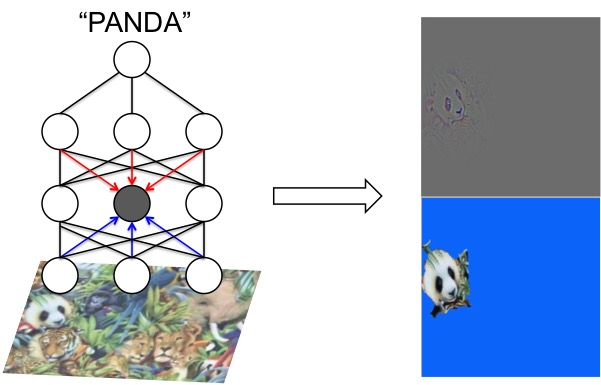
\includegraphics[width=0.95\columnwidth]{figs/splash0/splash}
% \vspace{-10pt}
\caption{We propose a novel Feedback Convolutional Net model for captuing visual attention by infering the status of hidden neuron activations. The feedback net is designed to utilize both bottom-up image features and top-down semantic labels to infer the hidden neuron activations. The salient area captured by feedback often matches the correponding "target" object, even in the images with cluttered background and multiple objects.}
\label{fig:splash0}
\vspace{-10pt}
\end{center}
\end{figure}

Visual attention typically is dominated by \emph{``goals''} from our mind easily in a top-down manner, especially in the case of object detection. Cognitive science explains this in the ``Biased Competition Theory''~\cite{beck2009top,desimone1998visual,desimone1995neural}, that human visual cortex is enhanced by top-down stimuli and non-relevant neurons will be suppressed in feedback loops when searching objects. By ``looking and thinking twice'', both human recognition and detection performances increase significantly especially in images with cluttered background~\cite{Cichy2014Resolving}. This leads to the selectivity in neuron activations~\cite{Kruger2013Deep}, which reduces the chance of recognition being interfered with either noises or distractive patterns.

Inspired by the above evidences, we present a novel \emph{Feedback Convolutional Neural Network} architecture in this paper. It achieves this selectivity by jointly reasoning the outputs of class nodes and the activations of hidden layer neurons during the feedback loop. As shown in Figure~\ref{fig:splash0}, during the feedforward stage, the proposed networks perform inference from image features in a bottom-up manner as traditional Convolutional Networks; while in feedback loops, it sets up high-level semantic labels (\emph{e.g.}, outputs of class nodes) as the ``goal'' in visual search to infer the activation status of hidden layer neurons. The networks are powerful enough to apply for class model visualization~\cite{simonyan2013deep, zeiler2014visualizing} and object localization even in cluttered scenes with multiple objects.

\setlength{\tabcolsep}{0.5pt}
\begin{figure*}[htb]
\begin{center}
\begin{tabular}{ccccccc}
%\rotatebox{90}{\hspace{5mm}Sequential} &
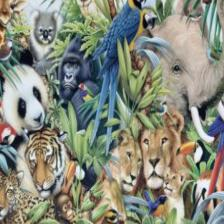
\includegraphics[width=0.14\linewidth]{figs/splash/original} &

\includegraphics[width=0.14\linewidth]{figs/splash/panda} &

\includegraphics[width=0.14\linewidth]{figs/splash/tiger} &
\includegraphics[width=0.14\linewidth]{figs/splash/gorilla} &
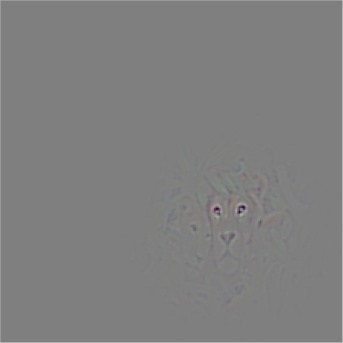
\includegraphics[width=0.14\linewidth]{figs/splash/lion} &

\includegraphics[width=0.14\linewidth]{figs/splash/elephant} &
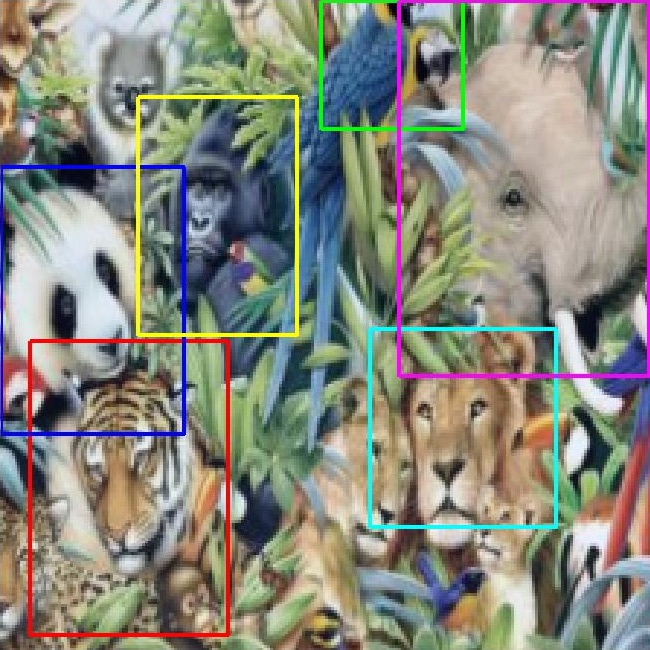
\includegraphics[width=0.14\linewidth]{figs/splash/localization}\\
{\small (a) Input Image} &
{\small (b) Panda} &
{\small (c) Tiger} &
{\small (d) Gorilla} &
{\small (e) Lion} &
{\small (f) Elephant} &
{\small (g) Localization}
\end{tabular}
% \vspace{-10pt}
\caption{We illustrate the localization power of the feedback net on a multi-object image with cluttered background. (a) shows the original input image which both VggNet and GoogleNet recongize as "comic book". (b) - (f) illustrate our feedback modelon understanding the image given different class labels as a prior. We visualize the gradient of each class node with respect to image after the feedback net finish its inference. (g) shows the final localizations for different objects based on the gradients. Better viewed in color.}
\label{fig:splah}
% \vspace{-30pt}
\end{center}
\end{figure*}

\subsection{Optimization in a Feedback Loop}
% Explain from the machine learning perspective
From a machine learning perspective, the proposed feedback networks \emph{add extra flexibility to Convolutional Networks, to help in capturing visual attention and improving feature detection}. Convolutional Neural Networks~\cite{lecun1998gradient, Krizhevsky2012ImageNet, Simonyan2014Very} have achieved great success in both machine learning and computer vision recent years. Benefit from large scale of training data, (\emph{e.g.,} ImageNet~\cite{deng2009imagenet}), CNNs are capable of learning filters and image compositions at the same time. Various approaches have been adopted to further increase ability of CNN, by either adding regularization in training~\cite{he2015delving,ioffe2015batch}, or going deeper~\cite{Simonyan2014Very, Szegedy2014Going}. Inspired by the Deformable Part-Based Models (DPM)~\cite{Felzenszwalb2010Object} that model middle level part locations as latent variables and search for them during object detection, we utilize a simple yet efficient method to optimize image compositions and assign neuron activations given ``goals'' in visual searching. The algorithm maximizes the posterior response of network given target high-level semantic concepts, in a top-down manner. Compared with traditional bottom-up strategies~\cite{he2015delving, ioffe2015batch} which aim to regularize the network training, the proposed feedback framework adds flexibilities to the model inference from high-level concepts down to receptive fields.

As the example shown in Figure~\ref{fig:splash0}, given a high-level semantic stimulus ``PANDA'', only the neurons in hidden layers related with the concept ``PANDA'' will be activated by iterative optimization in a feedback loop. As a result, only salient regions related with the concept ``PANDA'' are captured in visualizations. Figure~\ref{fig:splah} also shows the visualizations of saliencies given different semantic concepts for the same input image. As suggested by those results, the feedback networks achieve certain level of selectivity and provide non-relevant suppression during the top-down inference, allowing the model to focus on the most importatn image regions that improve the class confidence. 

%Comparisons between our method against two other visualization algorithms, Oxford~\cite{simonyan2013deep} and Deconvolution~\cite{zeiler2014visualizing}, are shown in Figure~\ref{fig:examples} in Section~\ref{sec:experiment}. Compared with state-of-the-arts, our feedback framework is capable to allow the model focusing on the most important image areas that improve the class confidence.

\subsection{Weakly Supervised Object Localization}
% Unify the network: recognition and detection in a single network.
% Simultaneously answer the question of "what" and "where"
Given the gradient visualizations shown in Figure~\ref{fig:splah}, we further develop an algorithm for weakly supervised object localization. Instead of using large amount of supervision (\emph{e.g.}, bounding box positions) in traditional methods such as R-CNN~\cite{girshick2014rich} or using regression model~\cite{erhan2014scalable, Simonyan2014Very}, we don't require any localization information in the training stage. In this case, we utilize \emph{a unified network performing both recognition and localization tasks}, to answer questions of ``what'' and ``where'' simultaneously, which are the two most important tasks in computer vision. Experimental results suggest that our weakly supervised algorithm using feedback network could achieve similar performance on ImageNet object localization task as GoogLeNet~\cite{Szegedy2014Going} and VGG~\cite{Simonyan2014Very}.

The remainder of this paper is organized as follows: Section~\ref{sec:related_work} introduces the related work, while we formulate our algorithm in Section~\ref{sec:model}. Experiments of visualization and object localization are demonstrated in Section~\ref{sec:experiment}. We conclude this work and future directions in Section~\ref{sec:conclusion}

% Implementation - caffe~\cite{jia2014caffe}



\begin{comment}

We present a novel feedback neural networks for joint reasoning the class node and hidden layer information. The network is powerful to be applied on model class visualization and object localization even in cluttered scenes with multi objects. The framework is novel and

\textbf{Deep Learning and Deep Convolutional Neural Networks, Feedforward Strcture}
Deep Convolutional networks (ConvNets) have recently enjoyed a great success in large-scale im- age and video recognition (Krizhevsky et al., 2012; Zeiler Fergus, 2013; Sermanet et al., 2014; Simonyan Zisserman, 2014) which has become possible due to the large public image reposito- ries, such as ImageNet (Deng et al., 2009), and high-performance computing systems, such as GPUs or large-scale distributed clusters (Dean et al., 2012). In particular, an important role in the advance of deep visual recognition architectures has been played by the ImageNet Large-Scale Visual Recog- nition Challenge (ILSVRC) (Russakovsky et al., 2014), which has served as a testbed for a few generations of large-scale image classification systems, from high-dimensional shallow feature en- codings (Perronnin et al., 2010) (the winner of ILSVRC-2011) to deep ConvNets (Krizhevsky et al., 2012) (the winner of ILSVRC-2012).

\textbf{Psychological feedback, inference top-down and bottom-up}
While we have outlined in this paper a hierarchical feedfor- ward view on visual processing, it is important to remember that within the visual cortex there are generally more feedback connections than forward connections. Also lateral connec- tions play an important role. This hints at the importance of processes like attention, expectation, top-down reasoning, imagination, and filling in. Many computer vision systems try to work in a purely feed-forward fashion. However, vision is inherently ambiguous and benefits from any prior knowledge available. This may even imply that the knowledge of how the tower of Pisa looks influences the perception of an edge on the level of V1. It also means that a system should be able to produce several hypotheses that are concurrently considered and possibly not resolved [102].

\textbf{This paper Main Contribution}
In this paper, we address the visualisation of deep image classification ConvNets, trained on the large-scale ImageNet challenge dataset [2]. To this end, we make the following three contributions. First, we demonstrate that understandable visualisations of ConvNet classification models can be ob- tained using the numerical optimisation of the input image [5] (Sect. 2). Note, in our case, unlike [5], the net is trained in a supervised manner, so we know which neuron in the final fully-connected clas- sification layer should be maximised to visualise the class of interest (in the unsupervised case, [9] had to use a separate annotated image set to find out the neuron responsible for a particular class). To the best of our knowledge, we are the first to apply the method of [5] to the visualisation of ImageNet classification ConvNets [8]. Second, we propose a method for computing the spatial support of a given class in a given image (image-specific class saliency map) using a single back-propagation pass through a classification ConvNet (Sect. 3). As discussed in Sect. 3.2, such saliency maps can be used for weakly supervised object localisation. Finally, we show in Sect. 4 that the gradient-based visualisation methods generalise the deconvolutional network reconstruction procedure [13].

\textbf{Yurgen's feedback neural networks, Attention neural networks, Deep Boltzman Machines}

\textbf{DPM  Top-down, weakly supervised object detection, localization and parsing}
We describe an object detection system that represents highly variable objects using mixtures of multiscale de- formable part models. These models are trained using a discriminative procedure that only requires bounding boxes for the objects in a set of images. The resulting system is both efficient and accurate, achieving state-of- the-art results on the PASCAL VOC benchmarks [11]– [13] and the INRIA Person dataset [10].
Our approach builds on the pictorial structures frame- work [15], [20]. Pictorial structures represent objects by a collection of parts arranged in a deformable configu- ration. Each part captures local appearance properties of an object while the deformable configuration is charac- terized by spring-like connections between certain pairs of parts.
Detections obtained with a single component person model. The model is defined by a coarse root filter (a), several higher resolution part filters (b) and a spatial model for the location of each part relative to the root (c). The filters specify weights for histogram of oriented gradients features. Their visualization show the positive weights at different orientations. The visualization of the spatial models reflects the “cost” of placing the center of a part at different locations relative to the root.

\textbf{Comparing against Oxford and Deconv}

\textbf{ConvNet Implementation Details}
ConvNet implementation details. Our visualisation experiments were carried out using a single deep ConvNet, trained on the ILSVRC-2013 dataset [2], which includes 1.2M training images, labelled into 1000 classes. Our ConvNet is similar to that of [8] and is implemented using their cuda-convnet toolbox1, although our net is less wide, and we used additional image jittering, based on zeroing-out random parts of an image. Our weight layer configuration is: conv64-conv256- conv256-conv256-conv256-full4096-full4096-full1000, where convN denotes a convolutional layer with N filters, fullM – a fully-connected layer with M outputs. On ILSVRC-2013 validation set, the network achieves the top-1/top-5 classification error of 39.7%/17.7%, which is slightly better than 40.7%/18.2%, reported in [8] for a single ConvNet.

\end{comment}

%\setlength{\tabcolsep}{2pt}
%\begin{figure*}
%\begin{center}
%\begin{tabular}{ccccccccc}
%\rotatebox{90}{\hspace{5mm}Oxford} &
%\includegraphics[width=0.11\linewidth]{figs/visual_compare/gradient/oxford/panda} &
%\includegraphics[width=0.11\linewidth]{figs/visual_compare/saliency/oxford/panda} &
%
\includegraphics[width=0.11\linewidth]{figs/visual_compare/gradient/oxford/tiger} &
%
\includegraphics[width=0.11\linewidth]{figs/visual_compare/saliency/oxford/tiger} &
%\includegraphics[width=0.11\linewidth]{figs/visual_compare/gradient/oxford/gorilla} &
%\includegraphics[width=0.11\linewidth]{figs/visual_compare/saliency/oxford/gorilla} &
%
\includegraphics[width=0.11\linewidth]{figs/visual_compare/gradient/oxford/lion} &
%
\includegraphics[width=0.11\linewidth]{figs/visual_compare/saliency/oxford/lion} \\
%\rotatebox{90}{\hspace{5mm}Deconv} &
%\includegraphics[width=0.11\linewidth]{figs/visual_compare/gradient/deconv/panda} &
%\includegraphics[width=0.11\linewidth]{figs/visual_compare/saliency/deconv/panda} &
%\includegraphics[width=0.11\linewidth]{figs/visual_compare/gradient/deconv/tiger} &
%\includegraphics[width=0.11\linewidth]{figs/visual_compare/saliency/deconv/tiger} &
%
\includegraphics[width=0.11\linewidth]{figs/visual_compare/gradient/deconv/gorilla} &
%
\includegraphics[width=0.11\linewidth]{figs/visual_compare/saliency/deconv/gorilla} &
%\includegraphics[width=0.11\linewidth]{figs/visual_compare/gradient/deconv/lion} &
%\includegraphics[width=0.11\linewidth]{figs/visual_compare/saliency/deconv/lion} \\
%\rotatebox{90}{\hspace{5mm}Our} &
%\includegraphics[width=0.11\linewidth]{figs/visual_compare/gradient/feedback/panda} &
%\includegraphics[width=0.11\linewidth]{figs/visual_compare/saliency/feedback/panda} &
%
\includegraphics[width=0.11\linewidth]{figs/visual_compare/gradient/feedback/tiger} &
%
\includegraphics[width=0.11\linewidth]{figs/visual_compare/saliency/feedback/tiger} &
%\includegraphics[width=0.11\linewidth]{figs/visual_compare/gradient/feedback/gorilla} &
%\includegraphics[width=0.11\linewidth]{figs/visual_compare/saliency/feedback/gorilla} &
%\includegraphics[width=0.11\linewidth]{figs/visual_compare/gradient/feedback/lion} &
%\includegraphics[width=0.11\linewidth]{figs/visual_compare/saliency/feedback/lion} \\
%&
%\multicolumn{2}{c}{{\small (a) Panda}} &
%\multicolumn{2}{c}{{\small (b) Tiger}} &
%\multicolumn{2}{c}{{\small (c) Gorilla}} &
%\multicolumn{2}{c}{{\small (d) Lion}} \\
%\end{tabular}
%% \vspace{-10pt}
%\caption{We demonstrate the effectiveness of our method by comparing the class model visualization results against Oxford~\cite{simonyan2013deep} and Deconv~\cite{zeiler2014visualizing}. The input image is the same as Figure 1 (a). We show both the visualization results as well as the saliency map. While both Oxford and Deconv have the same input: the image and an object class label (i.e. tiger, panda, etc.), the gradients computed are often salient on one particular object (i.e. elephant). Our feedback framework allows for the model to focus on the most important image area that improves the class confidence.}
%\label{fig:visual_compare}
%% \vspace{-30pt}
%\end{center}
%\end{figure*}

\section{Related Work}
\label{sec:related_work}

% Organization: 1) feedforward cnn 2) feedback network: RBM, Deconvolution, RNN. 3) visualization and attention 4) localization and detection
\subsection{Feedforward and Feedback Mechanism}
Deep Neural Network takes a \emph{feedforward-Back Error Propagation} strategy to learn features and classifiers simultaneously, from large scale of training samples~\cite{Krizhevsky2012ImageNet,Simonyan2014Very,lin2013network,salakhutdinov2009deep,bengio2013representation}. Various approaches have been proposed to further improve the discriminative ability of deep neural network, either by 1) adding regularization to improve the robustness of learnt model and get rid of overfitting, such as Dropout~\cite{srivastava2014dropout}, PReLU~\cite{he2015delving}, Batch Normalization~\cite{ioffe2015batch}; or 2) making the network deeper~\cite{Szegedy2014Going,Simonyan2014Very}.

Despite great successes achieved by applying Feedforward Networks to image recognition and detection, evidences accumulate from cognitive studies and point to the feedback mechanism that may dominant human perception processes~\cite{Cichy2014Resolving,Rust:2010if,Kruger2013Deep,lee2003hierarchical}. Recently, tentative efforts have been made to involve feedback strategy into Deep Neural Networks. Deep Boltzmman Machines (DBM)~\cite{salakhutdinov2009deep} and Deconvolutional Nerual Networks~\cite{Zeiler:2011hy} try to formulate the feedback as a reconstruction process within the training stage. Meanwhile, Recurrent Neural Networks (RNN) and Long Short Term Memory (LSTM)~\cite{hochreiter1997long} are utilized to capture the attention drifting in a dynamic environment and learn the feedback mechanisms via reinforcement learning~\cite{Stollenga:2014tl,Mnih:2014ti}. DRAW from Google DeepMind~\cite{gregor2015draw} combine above two into a generative model, to synthesis the image generation process.

As formulated in \emph{Biased Competition Theory}~\cite{beck2009top,desimone1995neural}, feedback, which passes the high-level semantic information down to the low-level perception, controls the selectivity of neuron activations in an extra loop in addition to the feedforward process. This results in the ``Top-Down'' attention in human cognition. Hierarchical probabilistic computational models~\cite{lee2003hierarchical} are proposed to characterize feedback stimuli in a top-down manner, which are further incorporated into deep neural networks, for example, modeling feedback loops as latent variables in DBM~\cite{wang2014attentional}, or using selectivity to resolve fine-grained classification~\cite{Mnih:2014ti}, \emph{et al.}. However, due to the computational efficiency and capacity limitations of generative models used in~\cite{Mnih:2014ti,wang2014attentional}, they are hardly used in large scale datasets.

\subsection{Visualization, Detection, and Localization}

Feedback is always related with visualization of CNN and object localization since both of these aim to project the high-level semantic information back to image representations. To visualize neuron responses and class models, various approaches are proposed either using deconvolution~\cite{zeiler2014visualizing} or optimization based on gradients~\cite{simonyan2013deep, le2013building}. As demonstrated in \cite{simonyan2013deep}, visualization of Convolutional Neural Network is showing semantically meaningful salient object regions and helps understand working mechanism of CNNs.

Object detection and localization are more about feedback, by treating detection / localization as a searching process with clear ``goals.'' To localize and detect objects in images, typical approaches use supervised training, which relies on large amount of supervision, \emph{e.g.}, ground-truth bounding boxes, or manually labeled segmentation in training samples~\cite{erhan2014scalable}. R-CNN~\cite{girshick2014rich} solves the detection problem by using region proposals instead of sliding windows. However, both of these approaches are computational intensive and naturally bottom-up: selecting candidate regions, performing feedforward classification and making decisions.

Inspired by visualizations of CNNs~\cite{zeiler2014visualizing,simonyan2013deep}, a more feasible and cognitive manner for detection / localization could be derived by utilizing the saliency maps generated in feedback visualizations. Moreover, an ideal approach should unify the recognition and detection in a single feedforward-feedback network architecture. However, the challenge lies on how to obtain semantically meaningful salience maps with high quality for each concept. That's the ultimate goal of our work presented in this paper.

\section{Model}
\label{sec:model}

\setlength{\tabcolsep}{2pt}
\begin{figure*}
\begin{center}
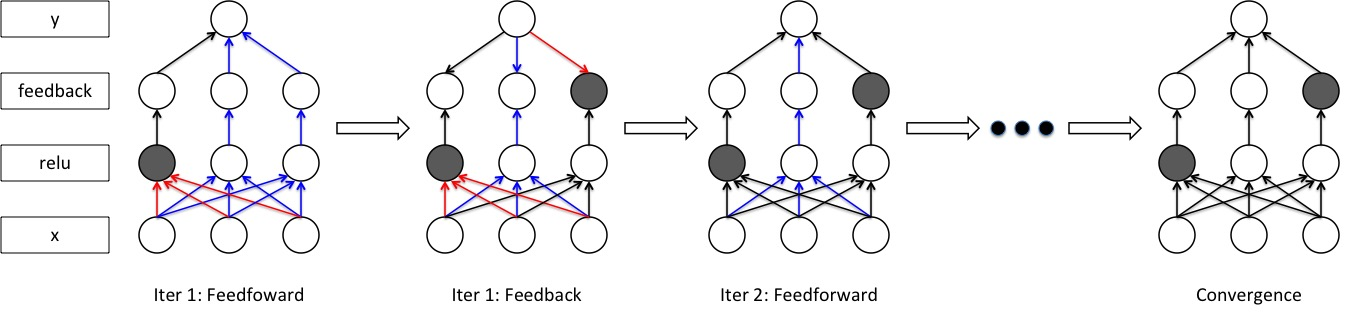
\includegraphics[width=0.95\linewidth]{figs/model/model}
% \vspace{-10pt}
\caption{Illustration of our feedback model and its inference process. At the first iteration, the model performs as a feedforward neural net. After then, the neurons in the feedback hidden layers update their activation status to maximize the confidence output of the target top neuron. This process continues until convergence. (We show only one layer here, but the feedback layers can be tacked in the deep ConvNet.) Better viewed in color.}
\label{fig:model}
% \vspace{-30pt}
\end{center}
\end{figure*}

We first review the current state-of-the-art feedforward Deep Convolutional Neural Networks (CNNs) architecture and then propose our feedback model.

\subsection{Review of Convolutional Neural Networks}
The most recent state-of-the-art deep CNNs~\cite{Simonyan2014Very} consist of many stacked feedforward layers, including convolutional, rectified linear units (ReLU) and max-pooling layers. For each layer, the input $\mathbf{x}$ can be an image or the output of a previous layer, consisting of $C$ input channels of width $M$ and height $N$: $\mathbf{x} \in \mathcal{R}^{M \times N \times C}$. The output $\mathbf{y}$ consists of a set of $C'$ output channels of width $M'$ and height $N'$: $\mathbf{y} \in \mathcal{R}^{M' \times N' \times C'}$.

\textbf{Convolutional Layer:}
The convolution layer is used to extract different features of the input. The convolutional layer is parameterized by $C'$ filters with every filter $\mathbf{k} \in \mathcal{R}^{K \times K \times C}$.
\begin{equation}
\mathbf{y}_{c'} = \sum_{c=1}^C \mathbf{k}_{c'c} * \mathbf{x}_c,\ \forall c'
\end{equation}

\textbf{ReLU Layer:}
The ReLU layer is used to increase the nonlinear properties of the decision function and of the overall network without affecting the receptive fields of the convoluional layer.
\begin{equation}
\mathbf{y} = \max (\mathbf{0}, \mathbf{x})
\label{eq:relu}
\end{equation}

\textbf{Max-Pooling Layer:}
The max-pooling layer is used to reduce the dimensionality of the output and variance in deformable objects to ensure that the same result will be obtained even when image features have small translations. The max-pooling operation is applied for every pixel $(i,j)$ around its small neighborhood $\mathcal{N}$.
\begin{equation}
y_{i,j,c} = \max_{u,v \in \mathcal{N}} x_{i+u, j+v, c},\ \forall i, j, c
\label{eq:max-pool}
\end{equation}

\begin{comment}
\textbf{Fully Connnected Layer:} The fully connected layer is parameterized by the production matrix with $W \in \mathcal{R}^{M'N'C' \times MNC}$.
Finally, a few fully connected layers (normally with drop-out) is stacked on top of the convolutional outputs to compute the scores of every class.
\begin{equation}
\vec{y}_l = W_l^T  \vec{y}_{l-1}
\end{equation}
\end{comment}

\subsection{Re-interpreting ReLU and Max-Pooling}
The ReLU and max-pooling layers can be re-interpreted as components for feature selection in neural nets. During feedforward computation, ReLU and max-pooling layers select those neuron signals that are either \emph{confident enough or locally maximal} to facilitate the invariance~\cite{riesenhuber1999hierarchical} and spatial assignments~\cite{weng1992cresceptron} for messages passing to higher levels.

We introduce a set of binary activation variables $\mathbf{z} \in \{0, 1\}$ to replace the $\max()$ operations in these layers. For the ReLU layer, $\mathbf{z}$ is the same size as the input $\mathbf{x}$ and Equation~\ref{eq:relu} can be rewritten as $\mathbf{y} = \mathbf{z} \circ \mathbf{x}$, where $\circ$ is the element wise product (Hadamard product). For the max-pooling layer, $\mathbf{z}$ is a set of convolutional filters except that they are location variant. Equation~\ref{eq:max-pool} can be rewritten as $\mathbf{y} = \mathbf{z} * \mathbf{x}$, where $*$ is the convolution operator.

For both layers, the $\max()$ functions are replaced with linear operations between the inputs and binary activation variables. The binary activation variables perform feature selection. However, the values of $\mathbf{z}$ are completely determined by the bottom-up input $\mathbf{x}$, meaning that the feature selections are purely based on bottom-up signals and won't be changed by any top-down information.

During the feedforward process, the neural nets need to keep an overall description of the image content and make image feature representations as general as possible, due to the lack of top-down semantic information. To achieve this target, middle-level neurons try to turn enough ReLUs on to avoid information loss; while the high-level fully connected layers are responsible for providing discriminability and descriptive ability. This works well when there is only one salient object in the image and no prior information is given. However, when the image contains multiple objects and complex scenes, the same feature may be too general to work equally well for all objects.

% During the feedforward process, the neural net features need to keep a overall description of the image content, due to the lack of top-down global information. The middle-level neurons try to turn on enough ReLU on while the high-level fully connected layers try to keep the feature embedding as discriminative and descriptive as possible. This works well when there is only one salient object in the image and no prior information is given. However, when the image contains multiple objects and complex scenes, the same feature may be too general to work equally well for all objects.

\subsection{Introducing the Feedback Layer}
Since the model opens all gates and allow maximal information getting through to ensure the generalization, to increase the discriminability within feature level, it is feasible to turn off those gates that provide irrelevant information when targeting at particular semantic labels. This strategy is explained as selectivity in biased competition theory~\cite{desimone1995neural} and is critical to realize the top-down attention.
%when we are targeted on a particular semantic labels, we want to turn off those gates that provide irrelevant information for seeing that object. This top-down message will be utilized to turn off those relu.

More technically, to increase the model flexibility to images and prior knowledges, we introduce an extra layer to the existing convolutional neural networks. We call it the feedback layer. The feedback layer contains another set of binary neuron activation variables $\mathbf{z} \in \{0, 1\}$, similar to ReLU's activation. However, these binary variables are activated according to the top-down message from outputs, instead of bottom inputs.
%
The feedback layer is stacked upon each ReLU layer, and they compose a hybrid control unit to active neuron response in both bottom-up and top-down manners:
\begin{description}
  \item[Bottom-Up] Inherent the selectivity from \emph{ReLU layers}, and the dominant features will be passed to upper layers;
  \item[Top-Down] Controlled by \emph{Feedback Layers}, which propagate the high-level semantics and global information back to image representation. This is achieved by activating only those gates related with target neurons.
\end{description}
% To further bring the model with the power of both bottom-up and top-down reasoning, we combine build the feedback layer on top of every ReLU layer. The ReLU gate will be open if bottom feature is significant enough while the feedback gate will open if the target neuron is significantly affected by the feature. The two layers together control the final gates for the message passing in the neural nets.
%
Figure.~\ref{fig:model} illustrates a simple architecture of our feedback model with only one ReLU layer and one feedback layer.

\subsection{Updating Hidden Neurons in Feedback Loops}
Given an image $I$ and a neural network with learned parameters $w$, we optimize the target neuron output by jointly inference on binary neuron activations $\mathbf{z}$ over all the hidden feedback layers. In particular, if the target neuron is a $k$-th class node in the top layer, we optimize the class score $s_k$ by re-adjusting the {\color{red} neuron activations} at every feedback layer $l$, channel $c$ and pixel $(i,j)$.
\begin{equation}
\begin{aligned}
& \max_\mathbf{z} & & s_k(I, \mathbf{z}) - \lambda ||\mathbf{z}|| \\
& s.t. & & \ z^l_{i,j,c} \in \{0, 1\}, \; \forall\ l, i, j, c
\end{aligned}
\end{equation}

This leads to an integer programming problem, which is NP-hard given the current deep net architecture. An approximated solution could be derived by applying a linear relaxation:
\begin{equation}
\begin{aligned}
& \max_\mathbf{z} & & s_k(I, \mathbf{z}) - \lambda ||\mathbf{z}|| \\
& s.t. & & \ 0 \leq z^l_{i,j,c} \leq 1, \; \forall\ l, i, j, c\\
\end{aligned}
\end{equation}

We use the gradient ascent algorithm to update the hidden variables through all layers simultaneously.
\begin{equation}
\begin{aligned}
\mathbf{z}_{t+1} = \mathbf{z}_t + \alpha \cdot (\frac{\partial s_k}{\partial \mathbf{z}} |_{\mathbf{z}_t} - \lambda)
\end{aligned}
\end{equation}

The initialization of feedback layer status $z$ is set to be the corresponding ReLU activation after the first feedforward pass and truncate $z$ when the updated values are either larger than 1 or smaller than 0 during inference.

\subsection{Implementation Details}
As for implementation details, we set the feedback layer on top of every ReLU layer except those taking the fully connected layers as inputs. It is suspected that the fully connected layers learn more embedding spaces rather than particular parts compared to convolutional layers. We set learning rate of hidden activations to 0.1 and update the neurons of all the feedback layers simultaneously. Each iteration performs a feedforward step of the neural net and a backpropagation step to send back gradients. This process usually converges in 10 to 50 iterations. The final {\color{red} neuron activations} are binarized by threshold $0.5$.

\section{Experimental Results}
\label{sec:experiment}

To verify the feedback model, we conduct qualitative experiments on class neuron visualizations and the weakly supervised object localization task. We use the three most popular pre-trained ConvNet models, AlexNet~\cite{Krizhevsky2012ImageNet}, VggNet~\cite{simonyan2013deep} and GoogleNet~\cite{Szegedy2014Going} for experiments. All three models are pre-trained with ImageNet 2012 classification training dataset~\cite{deng2009imagenet}, obtained from Caffe~\cite{jia2014caffe} model zoo. AlexNet achieves $\sim$15\% top 5 classification error on ImageNet 2012 testing dataset, while VggNet and GoogleNet obtains $\sim$7.5\%. GoogleNet slightly outperforms VggNet, but the gap is small and can be ignored.

\subsection{Image Specific Class Model Visualization}
\label{subsec:visualization}
Given an image $I$, a class label $k$ and the hidden neuron activation states $\mathbf{z}$, we approximate the neural net class score $s_k$ with the first-order taylor expansion in the neighborhood of $I$:
\begin{equation}
  s_k(I, \mathbf{z}) \approx  \mathbf{T}_k(\mathbf{z})^T I + b
\end{equation}
where $\mathbf{T}_k(\mathbf{z})$ is the derivative of $s_k$ with respect to the image at the point of $I$ and $\mathbf{z}$. $\mathbf{T}_k(\mathbf{z})$ can be viewed as the linear template applied on image $I$ for measuring how likely the image belongs to class $k$. We can visualize $\mathbf{T}$ since it's of the same size as the image $I$. We use this technique to visualize our feedback model throughout the paper.

Specifically, for a VggNet which uses a stack of piecewise linear layers (\emph{i.e.} Conv, ReLU and max-pooling) to compute the class scores, once the hidden states $\mathbf{z}$ are determined, the final score is a linear function of the image, which is equivalent to the inner product between the template and the image.

\textbf{Comparison of Visualization Methods:} We compare the image gradient (template $\mathbf{T}$) after the feedback process against the original one in feedforward pass, and Deconvolutional Neural Net (Deconv)~\cite{zeiler2014visualizing} on a set of complex images containing multiple objects from different classes. We show the qualititative results in Figure~\ref{fig:examples}. All techniques use the same pre-trained GoogleNet and ground truth class labels are given as a prior. The visualization results before feedback is the same as original image gradients, where all the hidden neurons states are determined by the bottom-up computations only, while visualizations turn out to be similar with Deconv after feedback. However, our feedback model captures more salient regions for the specific class while suppress irrelevant object areas much better than Deconv.

\textbf{Comparison of ConvNet Models:} We also qualitatively compare AlexNet, VggNet and Googlenet by visualizing their feedback templates in Figure~\ref{fig:model_compare}. All models are given ground truth class labels as a prior. From the visualization results, we find that VggNet and GoogleNet produce more accurate visual attention than AlexNet, suggesting that using smaller convolution filters and deeper architectures could further distinguish similar and nearby objects. We also observe that, although both VggNet and GoogleNet produce very smilar image classification accuracies, GoogleNet better captures the salient object areas than VggNet. We hypothesize that the two $4,096$ dimensional fully connected layers (\emph{i.e.}, fc6, fc7) in VggNet (which GoogleNet does not contain) could ruin the spatial distinctiveness of final image features, as pointed out in~\cite{lin2013network}.

\textbf{Feedback Visualization of Similar Classes:} We also show a few interesting feedback visualizations to help understand fine-grained classification models of GoogLeNet. The GoogLeNet is trained on ImageNet dataset with $1,000$ classes, among which there are $\sim$100 dog categories and $\sim$500 animal categories. We visualize the feedback templates of dog-cat images given particular dog classes and animal classes in Figure~\ref{fig:class_compare}. It is notable that each class has its own special salient image features for distinction. For example, some classes (\emph{i.e.} beagle, kit fox) look for local part features such as nose and ears, while others (\emph{i.e.} terrier, tiger) focus on global attributes such as furry and tabby.

\setlength{\tabcolsep}{0.5pt}
\begin{figure*}
\begin{center}
\begin{tabular}{ccccccc}
& \multicolumn{3}{c}{\small -------------------- Object 1: dog --------------------} & \multicolumn{3}{c}{\small -------------------- Object 2: cat --------------------} \\
\vspace{-2.5pt}
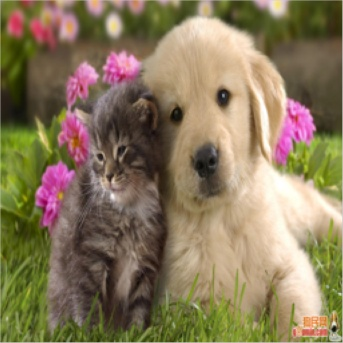
\includegraphics[width=0.14\linewidth,height=0.115\linewidth]{figs/examples/googlenet/oxford/dog-cat1} &
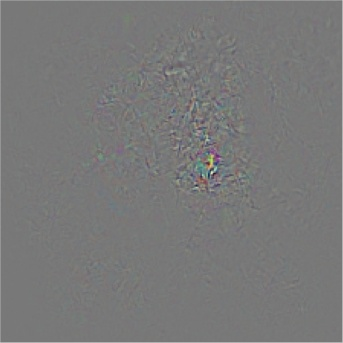
\includegraphics[width=0.14\linewidth,height=0.115\linewidth]{figs/examples/googlenet/oxford/dog-cat1_diff_258} &
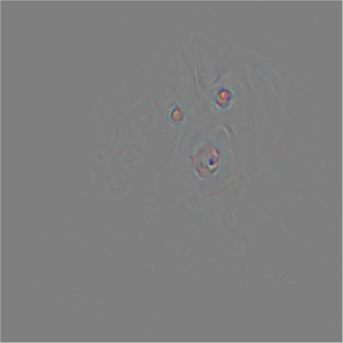
\includegraphics[width=0.14\linewidth,height=0.115\linewidth]{figs/examples/googlenet/deconv/dog-cat1_diff_258} &
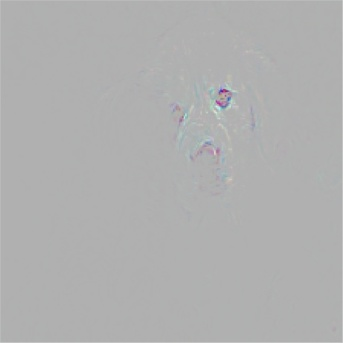
\includegraphics[width=0.14\linewidth,height=0.115\linewidth]{figs/examples/googlenet/soft/dog-cat1_diff_258} &
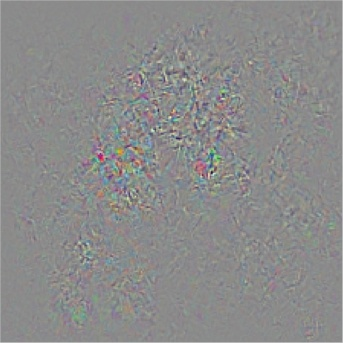
\includegraphics[width=0.14\linewidth,height=0.115\linewidth]{figs/examples/googlenet/oxford/dog-cat1_diff_286} &
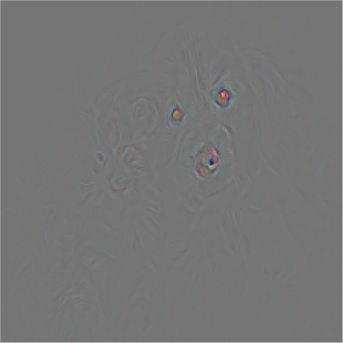
\includegraphics[width=0.14\linewidth,height=0.115\linewidth]{figs/examples/googlenet/deconv/dog-cat1_diff_286} &
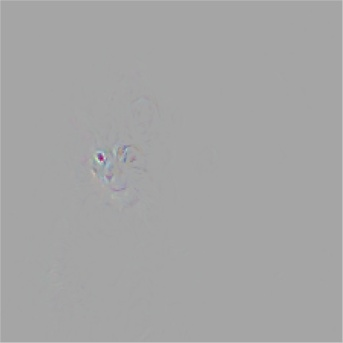
\includegraphics[width=0.14\linewidth,height=0.115\linewidth]{figs/examples/googlenet/soft/dog-cat1_diff_286} \\
\vspace{-2.5pt}
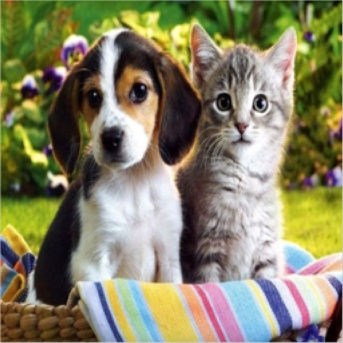
\includegraphics[width=0.14\linewidth,height=0.115\linewidth]{figs/examples/googlenet/oxford/dog-cat2} &
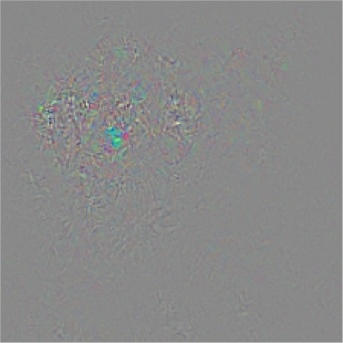
\includegraphics[width=0.14\linewidth,height=0.115\linewidth]{figs/examples/googlenet/oxford/dog-cat2_diff_163} &
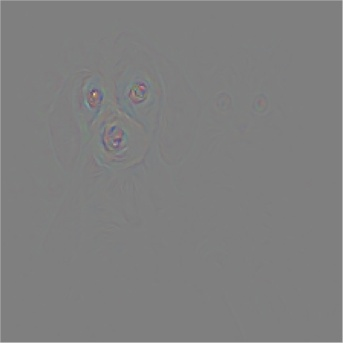
\includegraphics[width=0.14\linewidth,height=0.115\linewidth]{figs/examples/googlenet/deconv/dog-cat2_diff_163} &
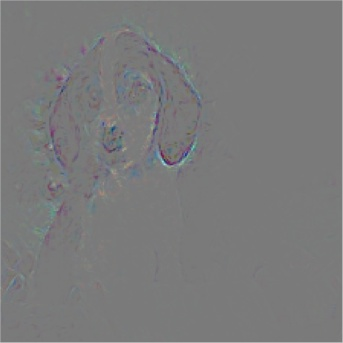
\includegraphics[width=0.14\linewidth,height=0.115\linewidth]{figs/examples/googlenet/soft/dog-cat2_diff_163} &
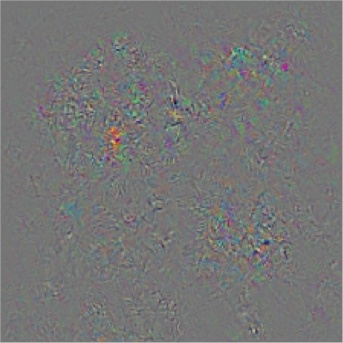
\includegraphics[width=0.14\linewidth,height=0.115\linewidth]{figs/examples/googlenet/oxford/dog-cat2_diff_286} &
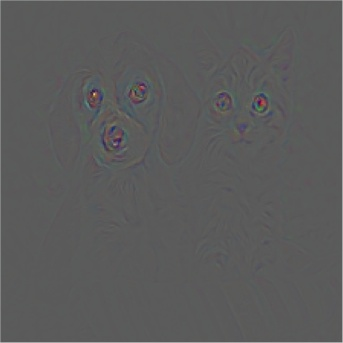
\includegraphics[width=0.14\linewidth,height=0.115\linewidth]{figs/examples/googlenet/deconv/dog-cat2_diff_286} &
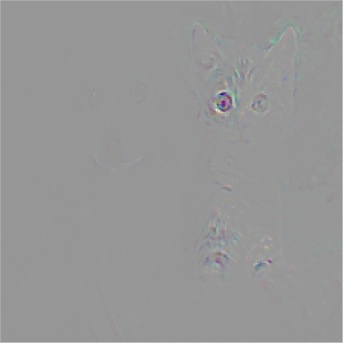
\includegraphics[width=0.14\linewidth,height=0.115\linewidth]{figs/examples/googlenet/soft/dog-cat2_diff_286} \\
\vspace{-2.5pt}
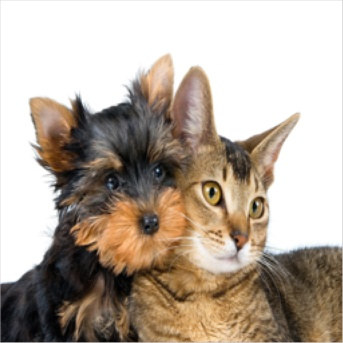
\includegraphics[width=0.14\linewidth,height=0.115\linewidth]{figs/examples/googlenet/oxford/dog-cat3} &

\includegraphics[width=0.14\linewidth,height=0.115\linewidth]{figs/examples/googlenet/oxford/dog-cat3_diff_188} &
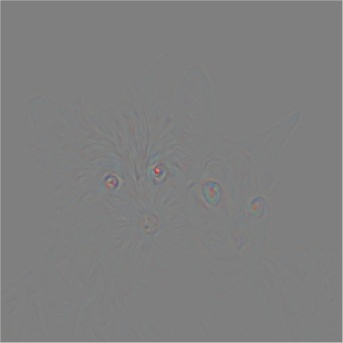
\includegraphics[width=0.14\linewidth,height=0.115\linewidth]{figs/examples/googlenet/deconv/dog-cat3_diff_188} &
\includegraphics[width=0.14\linewidth,height=0.115\linewidth]{figs/examples/googlenet/soft/dog-cat3_diff_188} &
\includegraphics[width=0.14\linewidth,height=0.115\linewidth]{figs/examples/googlenet/oxford/dog-cat3_diff_286} &
\includegraphics[width=0.14\linewidth,height=0.115\linewidth]{figs/examples/googlenet/deconv/dog-cat3_diff_286} &
\includegraphics[width=0.14\linewidth,height=0.115\linewidth]{figs/examples/googlenet/soft/dog-cat3_diff_286} \\
\vspace{-2.5pt}
\includegraphics[width=0.14\linewidth,height=0.115\linewidth]{figs/examples/googlenet/oxford/dog-cat4} &
\includegraphics[width=0.14\linewidth,height=0.115\linewidth]{figs/examples/googlenet/oxford/dog-cat4_diff_243} &
\includegraphics[width=0.14\linewidth,height=0.115\linewidth]{figs/examples/googlenet/deconv/dog-cat4_diff_243} &
\includegraphics[width=0.14\linewidth,height=0.115\linewidth]{figs/examples/googlenet/soft/dog-cat4_diff_243} &
\includegraphics[width=0.14\linewidth,height=0.115\linewidth]{figs/examples/googlenet/oxford/dog-cat4_diff_286} &
\includegraphics[width=0.14\linewidth,height=0.115\linewidth]{figs/examples/googlenet/deconv/dog-cat4_diff_286} &
\includegraphics[width=0.14\linewidth,height=0.115\linewidth]{figs/examples/googlenet/soft/dog-cat4_diff_286} \\
& \multicolumn{3}{c}{\small -------------------- Object 1: car --------------------} & \multicolumn{3}{c}{\small -------------------- Object 2: bike --------------------} \\
\vspace{-2.5pt}
\includegraphics[width=0.14\linewidth,height=0.115\linewidth]{figs/examples/googlenet/oxford/bic-car1} &
\includegraphics[width=0.14\linewidth,height=0.115\linewidth]{figs/examples/googlenet/oxford/bic-car1_diff_818} &
\includegraphics[width=0.14\linewidth,height=0.115\linewidth]{figs/examples/googlenet/deconv/bic-car1_diff_818} &
\includegraphics[width=0.14\linewidth,height=0.115\linewidth]{figs/examples/googlenet/soft/bic-car1_diff_818} &
\includegraphics[width=0.14\linewidth,height=0.115\linewidth]{figs/examples/googlenet/oxford/bic-car1_diff_672} &
\includegraphics[width=0.14\linewidth,height=0.115\linewidth]{figs/examples/googlenet/deconv/bic-car1_diff_672} &
\includegraphics[width=0.14\linewidth,height=0.115\linewidth]{figs/examples/googlenet/soft/bic-car1_diff_672} \\
\vspace{-2.5pt}
\includegraphics[width=0.14\linewidth,height=0.115\linewidth]{figs/examples/googlenet/oxford/bic-car2} &
\includegraphics[width=0.14\linewidth,height=0.115\linewidth]{figs/examples/googlenet/oxford/bic-car2_diff_818} &
\includegraphics[width=0.14\linewidth,height=0.115\linewidth]{figs/examples/googlenet/deconv/bic-car2_diff_818} &
\includegraphics[width=0.14\linewidth,height=0.115\linewidth]{figs/examples/googlenet/soft/bic-car2_diff_818} &
\includegraphics[width=0.14\linewidth,height=0.115\linewidth]{figs/examples/googlenet/oxford/bic-car2_diff_672} &
\includegraphics[width=0.14\linewidth,height=0.115\linewidth]{figs/examples/googlenet/deconv/bic-car2_diff_672} &
\includegraphics[width=0.14\linewidth,height=0.115\linewidth]{figs/examples/googlenet/soft/bic-car2_diff_672} \\
& \multicolumn{3}{c}{\small -------------------- Object 1: zebra --------------------} & \multicolumn{3}{c}{\small -------------------- Object 2: elephant --------------------} \\
\vspace{-2.5pt}
\includegraphics[width=0.14\linewidth,height=0.115\linewidth]{figs/examples/googlenet/oxford/zeb-ele1} &
\includegraphics[width=0.14\linewidth,height=0.115\linewidth]{figs/examples/googlenet/oxford/zeb-ele1_diff_341} &
\includegraphics[width=0.14\linewidth,height=0.115\linewidth]{figs/examples/googlenet/deconv/zeb-ele1_diff_341} &
\includegraphics[width=0.14\linewidth,height=0.115\linewidth]{figs/examples/googlenet/soft/zeb-ele1_diff_341} &
\includegraphics[width=0.14\linewidth,height=0.115\linewidth]{figs/examples/googlenet/oxford/zeb-ele1_diff_387} &
\includegraphics[width=0.14\linewidth,height=0.115\linewidth]{figs/examples/googlenet/deconv/zeb-ele1_diff_387} &
\includegraphics[width=0.14\linewidth,height=0.115\linewidth]{figs/examples/googlenet/soft/zeb-ele1_diff_387} \\
\includegraphics[width=0.14\linewidth,height=0.115\linewidth]{figs/examples/googlenet/oxford/zeb-ele2} &
\includegraphics[width=0.14\linewidth,height=0.115\linewidth]{figs/examples/googlenet/oxford/zeb-ele2_diff_341} &
\includegraphics[width=0.14\linewidth,height=0.115\linewidth]{figs/examples/googlenet/deconv/zeb-ele2_diff_341} &
\includegraphics[width=0.14\linewidth,height=0.115\linewidth]{figs/examples/googlenet/soft/zeb-ele2_diff_341} &
\includegraphics[width=0.14\linewidth,height=0.115\linewidth]{figs/examples/googlenet/oxford/zeb-ele2_diff_387} &
\includegraphics[width=0.14\linewidth,height=0.115\linewidth]{figs/examples/googlenet/deconv/zeb-ele2_diff_387} &
\includegraphics[width=0.14\linewidth,height=0.115\linewidth]{figs/examples/googlenet/soft/zeb-ele2_diff_387} \\
{\small (a) Image} &
{\small (b) Gradient} &
{\small (c) Deconv} &
{\small (d) Feedback} &
{\small (e) Gradient} &
{\small (f) Deconv} &
{\small (g) Feedback} \\
\end{tabular}
% \vspace{-10pt}
\caption{We demonstrate the effectiveness of feedback neural networks for class-specific feature extraction, by comparing the class model visualization results against original gradient~\cite{simonyan2013deep} and Deconv~\cite{zeiler2014visualizing} on selected images with multiple objects. All methods compute visualizations using a pre-trained GoogleNet trained on ImageNet 2012 classification dataset. Column (a) shows the input images (\emph{i.e.} dog v.s. cat, car v.s. bike, and zebra v.s. elephant). Column (b) and (e) show the original image gradients given the provided class labels. Column (c) and (f) show the Deconv results. Column (d) and (g) show the image gradients after feedback. Comparing against original gradient and Deconv, the feedback visualization captures more accurate salient area of the target object. For example, in the 4th row, both original template and Deconv see the dog and cat, even provided with the target label. In the last row, when zebra is specified, Deconv finds it hard to supress the elephant area. Our feedback method supress the irrelevant object much better. Better viewed in color and zoom in.}
\label{fig:examples}
% \vspace{-30pt}
\end{center}
\end{figure*}

\setlength{\tabcolsep}{0.5pt}
\begin{figure*}
\begin{center}
\begin{tabular}{ccccccc}
%\rotatebox{90}{\hspace{5mm}Gradient} &
\vspace{-2.5pt}
\includegraphics[width=0.14\linewidth,height=0.115\linewidth]{figs/examples/googlenet/soft/zeb-ele1} &
\includegraphics[width=0.14\linewidth,height=0.115\linewidth]{figs/examples/alexnet/soft/zeb-ele1_diff_341} &
\includegraphics[width=0.14\linewidth,height=0.115\linewidth]{figs/examples/vggnet/soft/zeb-ele1_diff_341} &
\includegraphics[width=0.14\linewidth,height=0.115\linewidth]{figs/examples/googlenet/soft/zeb-ele1_diff_341} &
\includegraphics[width=0.14\linewidth,height=0.115\linewidth]{figs/examples/alexnet/soft/zeb-ele1_diff_387} &
\includegraphics[width=0.14\linewidth,height=0.115\linewidth]{figs/examples/vggnet/soft/zeb-ele1_diff_387} &
\includegraphics[width=0.14\linewidth,height=0.115\linewidth]{figs/examples/googlenet/soft/zeb-ele1_diff_387} \\
%\rotatebox{90}{\hspace{5mm}Saliency} &
\vspace{-2.5pt}
\includegraphics[width=0.14\linewidth,height=0.115\linewidth]{figs/examples/googlenet/soft/zeb-ele1} &
\includegraphics[width=0.14\linewidth,height=0.115\linewidth]{figs/examples/alexnet/soft/zeb-ele1_sali_341} &
\includegraphics[width=0.14\linewidth,height=0.115\linewidth]{figs/examples/vggnet/soft/zeb-ele1_sali_341} &
\includegraphics[width=0.14\linewidth,height=0.115\linewidth]{figs/examples/googlenet/soft/zeb-ele1_sali_341} &
\includegraphics[width=0.14\linewidth,height=0.115\linewidth]{figs/examples/alexnet/soft/zeb-ele1_sali_387} &
\includegraphics[width=0.14\linewidth,height=0.115\linewidth]{figs/examples/vggnet/soft/zeb-ele1_sali_387} &
\includegraphics[width=0.14\linewidth,height=0.115\linewidth]{figs/examples/googlenet/soft/zeb-ele1_sali_387} \\
%\rotatebox{90}{\hspace{5mm}Gradient} &
\vspace{-2.5pt}
\includegraphics[width=0.14\linewidth,height=0.115\linewidth]{figs/examples/googlenet/soft/zeb-ele2} &
\includegraphics[width=0.14\linewidth,height=0.115\linewidth]{figs/examples/alexnet/soft/zeb-ele2_diff_341} &
\includegraphics[width=0.14\linewidth,height=0.115\linewidth]{figs/examples/vggnet/soft/zeb-ele2_diff_341} &
\includegraphics[width=0.14\linewidth,height=0.115\linewidth]{figs/examples/googlenet/soft/zeb-ele2_diff_341} &
\includegraphics[width=0.14\linewidth,height=0.115\linewidth]{figs/examples/alexnet/soft/zeb-ele2_diff_387} &
\includegraphics[width=0.14\linewidth,height=0.115\linewidth]{figs/examples/vggnet/soft/zeb-ele2_diff_387} &
\includegraphics[width=0.14\linewidth,height=0.115\linewidth]{figs/examples/googlenet/soft/zeb-ele2_diff_387} \\
%\rotatebox{90}{\hspace{5mm}Saliency} &
\includegraphics[width=0.14\linewidth,height=0.115\linewidth]{figs/examples/googlenet/soft/zeb-ele2} &
\includegraphics[width=0.14\linewidth,height=0.115\linewidth]{figs/examples/alexnet/soft/zeb-ele2_sali_341} &
\includegraphics[width=0.14\linewidth,height=0.115\linewidth]{figs/examples/vggnet/soft/zeb-ele2_sali_341} &
\includegraphics[width=0.14\linewidth,height=0.115\linewidth]{figs/examples/googlenet/soft/zeb-ele2_sali_341} &
\includegraphics[width=0.14\linewidth,height=0.115\linewidth]{figs/examples/alexnet/soft/zeb-ele2_sali_387} &
\includegraphics[width=0.14\linewidth,height=0.115\linewidth]{figs/examples/vggnet/soft/zeb-ele2_sali_387} &
\includegraphics[width=0.14\linewidth,height=0.115\linewidth]{figs/examples/googlenet/soft/zeb-ele2_sali_387} \\
%\rotatebox{90}{\hspace{5mm}Gradient} &
%\includegraphics[width=0.13\linewidth]{figs/examples/googlenet/soft/bic-car1} &
%\includegraphics[width=0.13\linewidth]{figs/examples/alexnet/soft/bic-car1_diff_818} &
%\includegraphics[width=0.13\linewidth]{figs/examples/vggnet/soft/bic-car1_diff_818} &
%\includegraphics[width=0.13\linewidth]{figs/examples/googlenet/soft/bic-car1_diff_818} &
%\includegraphics[width=0.13\linewidth]{figs/examples/alexnet/soft/bic-car1_diff_672} &
%\includegraphics[width=0.13\linewidth]{figs/examples/vggnet/soft/bic-car1_diff_672} &
%\includegraphics[width=0.13\linewidth]{figs/examples/googlenet/soft/bic-car1_diff_672} \\
%\rotatebox{90}{\hspace{5mm}Saliency} &
%\includegraphics[width=0.13\linewidth]{figs/examples/googlenet/soft/bic-car1} &
%\includegraphics[width=0.13\linewidth]{figs/examples/alexnet/soft/bic-car1_sali_818} &
%\includegraphics[width=0.13\linewidth]{figs/examples/vggnet/soft/bic-car1_sali_818} &
%\includegraphics[width=0.13\linewidth]{figs/examples/googlenet/soft/bic-car1_sali_818} &
%\includegraphics[width=0.13\linewidth]{figs/examples/alexnet/soft/bic-car1_sali_672} &
%\includegraphics[width=0.13\linewidth]{figs/examples/vggnet/soft/bic-car1_sali_672} &
%\includegraphics[width=0.13\linewidth]{figs/examples/googlenet/soft/bic-car1_sali_672} \\
%\rotatebox{90}{\hspace{5mm}Gradient} &
%\includegraphics[width=0.13\linewidth]{figs/examples/googlenet/soft/bic-car2} &
%\includegraphics[width=0.13\linewidth]{figs/examples/alexnet/soft/bic-car2_diff_818} &
%\includegraphics[width=0.13\linewidth]{figs/examples/vggnet/soft/bic-car2_diff_818} &
%\includegraphics[width=0.13\linewidth]{figs/examples/googlenet/soft/bic-car2_diff_818} &
%\includegraphics[width=0.13\linewidth]{figs/examples/alexnet/soft/bic-car2_diff_672} &
%\includegraphics[width=0.13\linewidth]{figs/examples/vggnet/soft/bic-car2_diff_672} &
%\includegraphics[width=0.13\linewidth]{figs/examples/googlenet/soft/bic-car2_diff_672} \\
%\rotatebox{90}{\hspace{5mm}Saliency} &
%\includegraphics[width=0.13\linewidth]{figs/examples/googlenet/soft/bic-car2} &
%\includegraphics[width=0.13\linewidth]{figs/examples/alexnet/soft/bic-car2_sali_818} &
%\includegraphics[width=0.13\linewidth]{figs/examples/vggnet/soft/bic-car2_sali_818} &
%\includegraphics[width=0.13\linewidth]{figs/examples/googlenet/soft/bic-car2_sali_818} &
%\includegraphics[width=0.13\linewidth]{figs/examples/alexnet/soft/bic-car2_sali_672} &
%\includegraphics[width=0.13\linewidth]{figs/examples/vggnet/soft/bic-car2_sali_672} &
%\includegraphics[width=0.13\linewidth]{figs/examples/googlenet/soft/bic-car2_sali_672} \\
{\small (a) Image} &
{\small (b) AlexNet} &
{\small (c) VggNet} &
{\small (d) GoogleNet} &
{\small (e) AlexNet} &
{\small (f) VggNet} &
{\small (g) GoogleNet} \\
\end{tabular}
% \vspace{-10pt}
\caption{We visualize the feedback ability of three most popular pre-trained ConvNets: AlexNet, VggNet and GoogleNet, by visualizing the final image gradients and salience maps after feedback. We show the input images in column (a). We show the results of the three models feedbacked by "zebra" in column (b), (c), (d) and by "elephant" in column (e), (f), (g) repsectively. We find that VggNet performs quite better than AlexNet, especially in capturing salient object details, suggesting the benefit of usage of small convolutional filters and deeper architecture. Although both VggNet and GogoleNet produce similar classification accruacy, we find GoogleNet provides the better class specific feature separations. We suspect the two 4096 fully connected layers in VggNet (which GoogleNetdoes not have) could harm the spatial distinctiveness of image features.}
\label{fig:model_compare}
% \vspace{-30pt}
\end{center}
\end{figure*}

\setlength{\tabcolsep}{0.5pt}
\begin{figure*}
\begin{center}
\begin{tabular}{ccccccc}
{\small (a) Image} &
{\small (b) G. pyrenees} &
{\small (c) Beagle} &
{\small (d) York. terrier} &
{\small (e) Kit fox} &
{\small (f) Tiger} &
{\small (g) Ostrich} \\
\vspace{-2.5pt}
&
\includegraphics[width=0.14\linewidth,height=0.08\linewidth]{figs/class_compare/pyrenees} &
\includegraphics[width=0.14\linewidth,height=0.08\linewidth]{figs/class_compare/beagle} &
\includegraphics[width=0.14\linewidth,height=0.08\linewidth]{figs/class_compare/yorkshire-terrier} &
\includegraphics[width=0.14\linewidth,height=0.08\linewidth]{figs/class_compare/kit-fox} &
\includegraphics[width=0.14\linewidth,height=0.08\linewidth]{figs/class_compare/tiger} &
\includegraphics[width=0.14\linewidth,height=0.08\linewidth]{figs/class_compare/ostrich} \\
\vspace{-2.5pt}
\includegraphics[width=0.14\linewidth,height=0.115\linewidth]{figs/class_compare/googlenet/soft/dog-cat1} &
\includegraphics[width=0.14\linewidth,height=0.115\linewidth]{figs/class_compare/googlenet/soft/dog-cat1_diff_258} &
\includegraphics[width=0.14\linewidth,height=0.115\linewidth]{figs/class_compare/googlenet/soft/dog-cat1_diff_163} &
\includegraphics[width=0.14\linewidth,height=0.115\linewidth]{figs/class_compare/googlenet/soft/dog-cat1_diff_188} &
\includegraphics[width=0.14\linewidth,height=0.115\linewidth]{figs/class_compare/googlenet/soft/dog-cat1_diff_279} &
\includegraphics[width=0.14\linewidth,height=0.115\linewidth]{figs/class_compare/googlenet/soft/dog-cat1_diff_293} &
\includegraphics[width=0.14\linewidth,height=0.115\linewidth]{figs/class_compare/googlenet/soft/dog-cat1_diff_10} \\
\vspace{-2.5pt}
\includegraphics[width=0.14\linewidth,height=0.115\linewidth]{figs/class_compare/googlenet/soft/dog-cat2} &
\includegraphics[width=0.14\linewidth,height=0.115\linewidth]{figs/class_compare/googlenet/soft/dog-cat2_diff_258} &
\includegraphics[width=0.14\linewidth,height=0.115\linewidth]{figs/class_compare/googlenet/soft/dog-cat2_diff_163} &
\includegraphics[width=0.14\linewidth,height=0.115\linewidth]{figs/class_compare/googlenet/soft/dog-cat2_diff_188} &
\includegraphics[width=0.14\linewidth,height=0.115\linewidth]{figs/class_compare/googlenet/soft/dog-cat2_diff_279} &
\includegraphics[width=0.14\linewidth,height=0.115\linewidth]{figs/class_compare/googlenet/soft/dog-cat2_diff_293} &
\includegraphics[width=0.14\linewidth,height=0.115\linewidth]{figs/class_compare/googlenet/soft/dog-cat2_diff_10} \\
\includegraphics[width=0.14\linewidth,height=0.115\linewidth]{figs/class_compare/googlenet/soft/dog-cat3} &
\includegraphics[width=0.14\linewidth,height=0.115\linewidth]{figs/class_compare/googlenet/soft/dog-cat3_diff_258} &
\includegraphics[width=0.14\linewidth,height=0.115\linewidth]{figs/class_compare/googlenet/soft/dog-cat3_diff_163} &
\includegraphics[width=0.14\linewidth,height=0.115\linewidth]{figs/class_compare/googlenet/soft/dog-cat3_diff_188} &
\includegraphics[width=0.14\linewidth,height=0.115\linewidth]{figs/class_compare/googlenet/soft/dog-cat3_diff_279} &
\includegraphics[width=0.14\linewidth,height=0.115\linewidth]{figs/class_compare/googlenet/soft/dog-cat3_diff_293} &
\includegraphics[width=0.14\linewidth,height=0.115\linewidth]{figs/class_compare/googlenet/soft/dog-cat3_diff_10} \\
\end{tabular}
% \vspace{-10pt}
\caption{We show some interesting visualizations for the understanding of fine-grained classification by comparsing against the feedback gradients of ground truth labels and other classes. The top row shows the class labels and a representative image for each class for the ease of understanding. Column (a) shows the three examplar input images, their ground truth labels are great pyrenees, beagle and yorkshire terrier respectively. We can see that although (b), (c) and (d) are all dogs, their salient area for distinction are quite different. Noses are one of the most important feature for classifying dogs, but ears are specific feature for beagles, while fluffy is more importatnt to yorkshire terrier. When the top down is from (e) kit fox, features on the cat in the last row is more fox-specific: nose and ears. When top down is from (f) tiger, features on the same at is more tiger-specific: textures. And when it's (g) ostrich, nothing special come out.}
\label{fig:class_compare}
% \vspace{-30pt}
\end{center}
\end{figure*}

\subsection{Weakly Supervised Object Localization}
\label{subsec:localization}
To quantitatively demonstrate the effectiveness of the feedback model. we experiment on the ImageNet 2014 localization task.

As pointed in~\cite{simonyan2013deep}, the magnitude of the elements in the model template $\mathbf{T}_k$ defines the class specific salience map on image $I$. Pixels with larger magnitudes indicate that they are more important to the class. We adopt the same saliency extraction strategy as~\cite{simonyan2013deep} that a single class saliency value $M_k$ for class $k$ at pixel $(i,j)$ is computed across all color channels: $M_k(i,j) = \max_{c \in rgb} | T_k(i,j,c) |$.

We show that the proposed Feedback CNN has to potential to unify recognition and detection into a single network architecture in this experiment, instead of using separate ones to perform different tasks respectively. Although the three ConvNets are pre-trained for image classification, we could use the feedbacked salience map for weakly supervised object localization. Following~\cite{simonyan2013deep}, given an image and the corresponding class salience map, we compute the object segmentation mask using the GraphCut color image segmentation~\cite{yuri2001interactive}. To initialize graph cut, we treat pixels with saliency higher than 95\% quantile of the saliency distribution in the image as foreground and those lower than 30\% quantile as background. Once foreground and background segmentations are computed, the object segmentation mask is set to be the largest connected foreground component, and the tightest bounding box is extracted as the localization result.

We test our localization results on ImageNet 2014 localization validation set, which contains $\sim20,000$ images with each image associated with labels and corresponding bounding boxes. A prediction is considered as correct if its overlap with the ground truth bounding box is over 50\%. Image are resized  to 224x224 to meet the model requirement on resolutions, and ground-truth class labels are provided to predict localizations. Neither further preprocessing nor multi-scale strategy are involved.

\textbf{Comparison of Localization Methods:} Table~\ref{tab:localization_accuracy} shows the comparison of our weakly supervised localization accuracy against the baseline method~\cite{simonyan2013deep}. For fair comparison, we reimplemented the method in~\cite{simonyan2013deep} following the details in the original paper strictly, and name as ``Oxford.'' For our own method, we use GoogLeNet and apply the same segmentation strategy in our model. Our method obtains 38.8\% localization error, significantly outperforming Oxford 44.6\%, suggesting that in terms of capturing attention and localizing salient objects, our feedback net is better. Note that our weakly supervised localization error is even closer to a carefully trained supervised localization model (34.3\%).

\textbf{Comparsion of ConvNet Models:} We also analyze  weakly supervised localization accuracies of above mentioned three ConvNets in Table~\ref{tab:localization_model_compare}, provided with the same testing protocol. Even provided with ground truth class, VggNet and GoogleNet significantly outperforms AlexNet.
This suggests that better feature representations are sharable between the two highly correlated visual tasks: recognition and localization. GoogLeNet outperforms VggNet even further, which matches the observations in Figure~\ref{fig:model_compare}.

%\textbf{Comparsion of ConvNet Models:} We also analyze the weakly supervised localization accuracy of the three ConvNets in Table~\ref{tab:localization_model_compare}, provided with the same testing protocol. Even provided with ground truth class, VggNet and GoogleNet significantly outperforms AlexNet, suggesting that better feature representations are sharable between the two highly correlated visual tasks: recognition and localization. GoogleNet outperforms VggNet even further, which matches the observations in Figure~\ref{fig:model_compare}.

%However, Most of the images in ImageNet 2014 dataset contain only one salient object. We further show some localization results on images with multiple object classes in Figure~\ref{} ... \textbf{\color{red} I need the figures to complete the paragraph}. Obviously our feedback net cannot distinguish multiple object instances from the same class, but could capture the salient areas, which could be utilized by other sophisticated object detection algorithms.

\begin{table}
\centering
\small
Localization Errors Given Ground Truth Labels
\begin{tabular}{|c|c|}
\hline
Method & Localization Error (\%) \\ \hline
Oxford~\cite{simonyan2013deep} & 44.6 \\ \hline
%Deconv~\cite{zeiler2014visualizing} & 46.9 \\ \hline
Feedback & \textbf{38.8} \\ \hline
Oxford-Supervised~\cite{Simonyan2014Very} & 34.3 \\ \hline
\end{tabular}
\caption{We compare our weakly supervised localization results on ImageNet 2014 validation set with the simplified testing protocol: the bounding box is predicted from a single central crop of images and the ground truth labels are provided. We show that our feedback method siginificantly outperforms the baseline method (44.6\%) that uses the original image gradient to localize, and works even closer to a carefully trained supervised localization model (34.3\%).}
\label{tab:localization_accuracy}
\end{table}

\begin{table}
\centering
\small
Localization Errors of Different Feedback ConvNets
\begin{tabular}{|c|c|}
\hline
Model & Localization Error (\%) \\ \hline
AlexNet~\cite{Krizhevsky2012ImageNet} & 49.6 \\ \hline
VggNet~\cite{Simonyan2014Very} & 40.2 \\ \hline
GooglNet~\cite{Szegedy2014Going} & \textbf{38.8} \\ \hline
\end{tabular}
\caption{We analyze the attention ability by running our feedback mechanism on the three popular ConvNets. All models use the same testing protocol as Table~\ref{tab:localization_accuracy}. Even provided with ground truth class, VggNet and GoogleNet significant outperforms AlexNet suggesting they are learning better features. GoogleNet outperforms VggNet even further, which matches the observations in Figure~\ref{fig:model_compare}.}
\label{tab:localization_model_compare}
\end{table}

%\begin{table}
%\centering
%Localization Error With Top 5 Predictions
%\begin{tabular}{|c|c|c|c|} \hline
%Method & AlexNet & VggNet & GoogleNet \\ \hline
%Oxford~\cite{simonyan2013deep} & 53.4 & 51.6 & 47.8 \\ \hline
%Deconv~\cite{zeiler2014visualizing} & 55.2 & 52.2 & 49.6\\ \hline
%Feedback & 52.3 & 49.0 & \textbf{46.1} \\ \hline
%\end{tabular}
%\caption{We compare the localization results on ImageNet 2014 validation set against Oxford and Deconv, using three different ConvNet models. Our feedback method clearly outperforms the baseline approaches for weakly supervised object localization. Notably, although VggNet and GoogleNet have ery similar image classfication accuray on ImageNet, our comparison suggests GoogleNet learns better middle level features than VggNet.}
%\label{tab:localization_accuracy_top5}
%\end{table}

\section{Conclusion \& Discussion}
\label{sec:conclusion}

We propose a Feedback Convolutional Neural Network architecture in this paper, which achieves the selectivity of neuron activations by jointly reasoning the outputs of class nodes and the activations of hidden layer neurons during the feedback loop. The proposed Feedback CNN is capable of capturing high level semantic concepts and project the information down to image representation as salience maps. Benefiting from the feedback mechanism of our model, we utilize the salience map to build a unified deep neural network for both recognition and object localization tasks, to answer questions of both ``What'' and ``Where'' simultaneously. Experimental results on ImageNet 2014 object localization Challenge show that our model could achieve competitive performance compared with state-of-the-arts, using only weakly supervised information.

%The Feedback CNNs have the potential to further improve various computer vision and machine learning tasks, such as fine-grained recognition, multi-task learning, and object detection. While they may also help training better CNN models with semi-supervised learning. We leave these topics as future work. 

% Finally, I wrote down this sentence and comment it. It will make sense, but may not be suitable to put it here.
% In the meanwhile, we are also wondering how human perception and cognitive mechanism would help in computer vision and machine learning. Instead of simulating the human vision system, building an efficient computational model that works for computer is more promising.

\begin{comment}
We proposes a Feedback Convolusional Neural Networks for class model visualization and object localization.
Our Feedback Neural Networks can infer the hidden neuron status given the bottom level input image and top level class labels.
Experiments on ImageNet localization challengeindicates that our model is superior in weakly supervised object localization, and further experiments demonstrate its powerfulness in distinguishing objects, even under cluttered backgrounds with multiple objects.

(1) Robust
(2) Multi-task
(3)

Figure 1: We show the powerfulness of feedback neural networks on class model visualization and object localizations, even when an image contains very cluttered background and lots of salient objects. Note that we simply use a pertained feedforward multi-class convnets (GoogleNet) model [] trained with ImageNet dataset where each training image only contains one object and no further training is involved. The feedback neural nets are able to adapt its middle-level hidden layers (usually represents object parts) by combining the bottom-up feedforward image features as well as top-down feedback semantic information. (a) input image (b) class model visualization given the class label: panda, elephant, gorilla, tiger, lion, (c) final object localization results based on the class model visualization.
\end{comment}


{\small
\bibliographystyle{ieee}
\bibliography{egbib}
}

\end{document}
